\setcounter{equation}{0}
\section{Quantum Computation}

We are concerned with using quantum computation to produce solutions to problems which are considered intractable for classical computers. \footnote { An \emph{intractable} problem is one for which execution time grows exponentially as input size increases linearly.} To see how quantum computers can compute classically intractable problems, we need to examine how they perform computation.

The building block of the quantum computer is the \emph{qubit}, or quantum bit. A qubit is an abstract value, represented by nano scale properties of physical matter. Qubits have been implemented using ion charge, photon polarization, nuclear spin of atoms, and nuclear spin of impurities in silicon chips.

Classical bits abstractly represent values of 0 or 1 by the absence or presence of voltage. In contrast , a qubit represents both a 0 and 1 simultaneously due to superposition.

Since qubits represent two values at once, \emph{n} qubits represent $2^n$ values. Thus, quantum computers operate on exponential data with only linear input. For example: two qubits represent the values 00 01 10 and 11 simultaneously. The probability of the value which will be observed is represented by a complex number called \emph{probability amplitude}.

Probability amplitudes are mathematically analogous to a wave: they can be positive or negative, and are subject to interference. The probability amplitude of a value is the sum of probability amplitudes over all entangled particles. The classical probability of a value is given by the square of its probability amplitude. Quantum computation is performed by manipulating probability amplitudes of qubits.

A qubit can be represented by unit vector in the Hilbert space $C^2$, where C is the set of complex numbers. An n-qubit system can be described by the tensor product of these Hilbert spaces:

%formul

We can compute a function f on these qubits by applying a unitary operator \emph{U}:

%formul

when f is one-to-one, ie reversible, we can always find a unitary operator. Any classical function we wish to compute can be made reversible using extra bits and acceptable operational overhead. We can think of \emph{U} as a basic quantum gate, performing the role of a classical truth table. We can represent \emph{U} as a unitary matrix, which by definition is reversible.

To apply \emph{U} and thereby compute our function \emph{f}, we find the Hamiltonian \emph{H} which solves the equation :

%formul

Absolution exists as long as \emph{U} is unitary. By applying \emph{U} to a vector on \emph{n} qubits we apply \emph{f} to all possible $2^n$ inputs in parallel. This parallelism is how quantum computation overcomes classically intractable problems.

Obtaining the computed solution presents a new challenge. The superposition of n qubits have $2^n$ possible states, and is called a \emph{wave} function. By observing the value of a vector of qubits we \emph{collapse} this wave function, selecting one state from exponentially many to produce a classical bit vector.
This collapsing effectively destroys the solution. However, we can use the interference property of probability of observing the correct answer.

Quantum computing is not without drawbacks. Firstly, the exponential parallelism inherent in quantum computation does not imply exponential computational power. In addition, practical implementation is hindered by decoherence, caused by interference from the environment as well as the exponential decay times of quantum states. Quantum error correcting codes are necessary to mitigate decoherence and error propagation in the real world. These
codes require many physical qubits to accurately encode a single logical qubit of information. Finally, certain quantum architectures have impractical requirements, such as operating at near absolute zero temperature. Current quantum computers require classical control components, and CMOS transistors cannot be used in such an environment.

Due to these difficulties, simulation is important for the development and advancement of quantum algorithms. Quantum simulators run on classical computers and allow state observation, analysis of error accumulation, and feasibility studies. However, simulating a $2^n$ dimensional Hilbert space on a classical system requires manipulating bit vectors of size $2^n$, whereas quantum computers need only \emph{n} qubits. As a result, quantum simulators are restricted to small numbers of qubits.

Real quantum computers do exist which operate on 5-7 qubits. Shor's algorithm was successfully demonstrated on a 7-qubit machine. 

\begin{figure}
\begin{center}
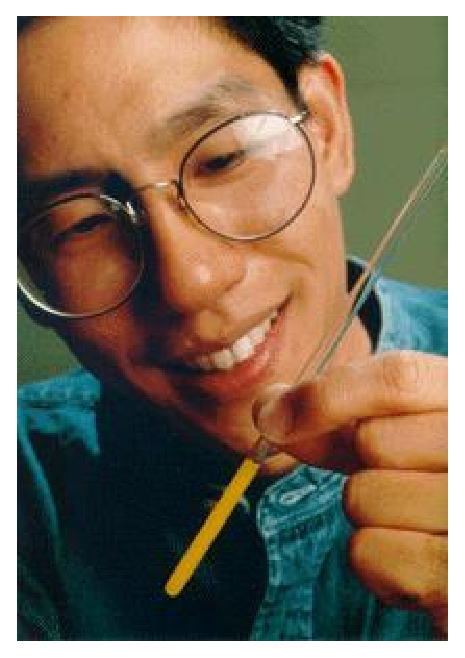
\includegraphics{20000815_chuang_vial}
\end{center}
\label{IBM'S 5 qubit quantum computer}
\caption{ Dr. Isaac Chuang, research staff member at IBM's Almaden Research Center (San Jose, Calif.), holds a quantum computer -- a glass tube containing specially designed molecules that can solve some of the most difficult mathematical problems exponentially faster than a conventional computer. }
\end{figure}

